% Created by tikzDevice version 0.12 on 2019-03-05 08:06:15
% !TEX encoding = UTF-8 Unicode
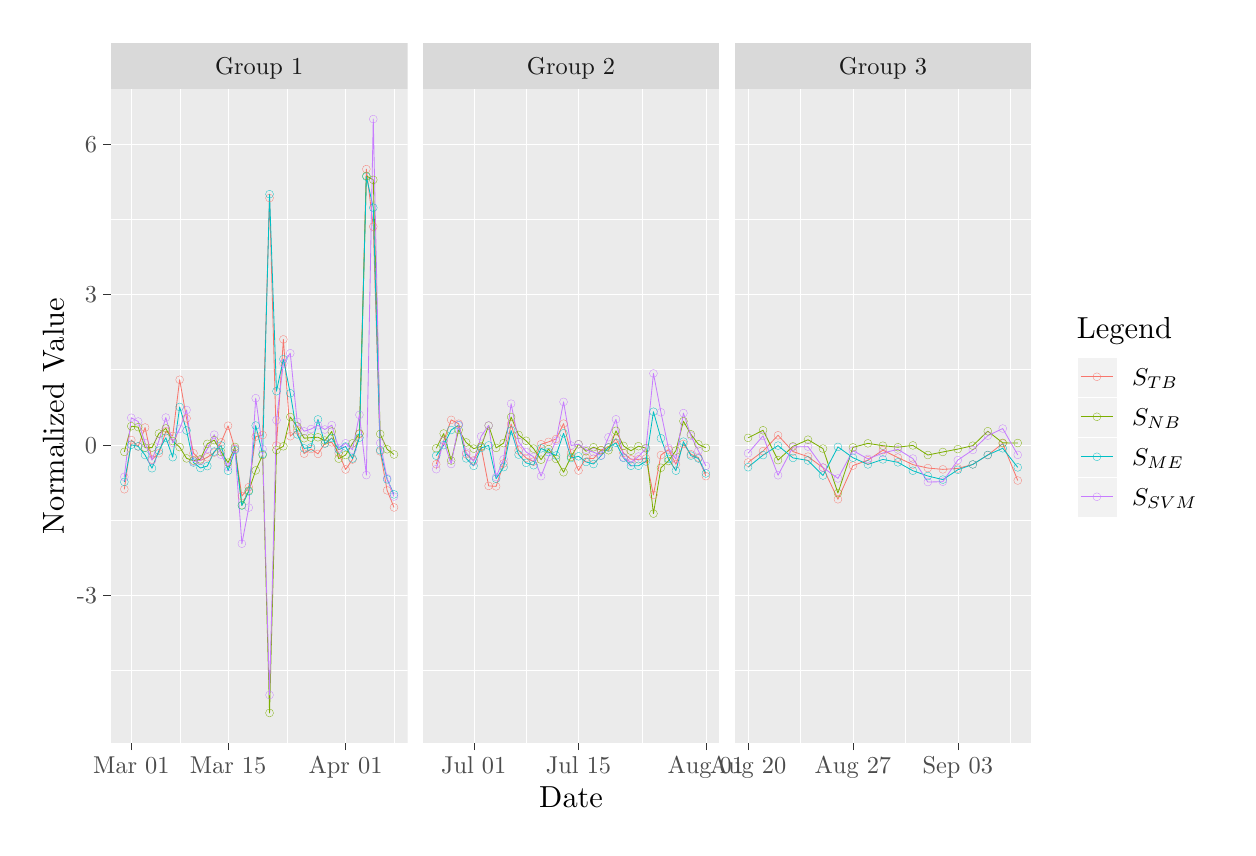
\begin{tikzpicture}[x=1pt,y=1pt]
\definecolor{fillColor}{RGB}{255,255,255}
\path[use as bounding box,fill=fillColor,fill opacity=0.00] (0,0) rectangle (433.62,289.08);
\begin{scope}
\path[clip] (  0.00,  0.00) rectangle (433.62,289.08);
\definecolor{drawColor}{RGB}{255,255,255}
\definecolor{fillColor}{RGB}{255,255,255}

\path[draw=drawColor,line width= 0.1pt,line join=round,line cap=round,fill=fillColor] (  0.00,  0.00) rectangle (433.62,289.08);
\end{scope}
\begin{scope}
\path[clip] ( 30.06, 30.73) rectangle (137.25,266.77);
\definecolor{fillColor}{gray}{0.92}

\path[fill=fillColor] ( 30.06, 30.73) rectangle (137.25,266.77);
\definecolor{drawColor}{RGB}{255,255,255}

\path[draw=drawColor,line width= 0.1pt,line join=round] ( 30.06, 56.94) --
	(137.25, 56.94);

\path[draw=drawColor,line width= 0.1pt,line join=round] ( 30.06,111.24) --
	(137.25,111.24);

\path[draw=drawColor,line width= 0.1pt,line join=round] ( 30.06,165.53) --
	(137.25,165.53);

\path[draw=drawColor,line width= 0.1pt,line join=round] ( 30.06,219.83) --
	(137.25,219.83);

\path[draw=drawColor,line width= 0.1pt,line join=round] ( 54.92, 30.73) --
	( 54.92,266.77);

\path[draw=drawColor,line width= 0.1pt,line join=round] ( 93.65, 30.73) --
	( 93.65,266.77);

\path[draw=drawColor,line width= 0.1pt,line join=round] (132.37, 30.73) --
	(132.37,266.77);

\path[draw=drawColor,line width= 0.1pt,line join=round] ( 30.06, 84.09) --
	(137.25, 84.09);

\path[draw=drawColor,line width= 0.1pt,line join=round] ( 30.06,138.38) --
	(137.25,138.38);

\path[draw=drawColor,line width= 0.1pt,line join=round] ( 30.06,192.68) --
	(137.25,192.68);

\path[draw=drawColor,line width= 0.1pt,line join=round] ( 30.06,246.98) --
	(137.25,246.98);

\path[draw=drawColor,line width= 0.1pt,line join=round] ( 37.43, 30.73) --
	( 37.43,266.77);

\path[draw=drawColor,line width= 0.1pt,line join=round] ( 72.41, 30.73) --
	( 72.41,266.77);

\path[draw=drawColor,line width= 0.1pt,line join=round] (114.88, 30.73) --
	(114.88,266.77);
\definecolor{drawColor}{RGB}{248,118,109}

\path[draw=drawColor,line width= 0.3pt,line join=round] ( 34.93,122.29) --
	( 37.43,140.08) --
	( 39.93,137.74) --
	( 42.42,144.59) --
	( 44.92,133.03) --
	( 47.42,135.31) --
	( 49.92,143.23) --
	( 52.42,141.55) --
	( 54.92,161.86) --
	( 57.42,147.90) --
	( 59.91,135.32) --
	( 62.41,132.68) --
	( 64.91,133.83) --
	( 67.41,135.55) --
	( 69.91,139.26) --
	( 72.41,145.23) --
	( 74.91,136.85) --
	( 77.40,119.81) --
	( 79.90,123.04) --
	( 82.40,141.30) --
	( 84.90,141.87) --
	( 87.40,227.52) --
	( 89.90,138.12) --
	( 92.40,176.45) --
	( 94.89,141.46) --
	( 97.39,143.64) --
	( 99.89,135.15) --
	(102.39,136.82) --
	(104.89,135.06) --
	(107.39,138.90) --
	(109.89,139.25) --
	(112.39,135.37) --
	(114.88,129.44) --
	(117.38,133.04) --
	(119.88,142.23) --
	(122.38,237.97) --
	(124.88,217.18) --
	(127.38,135.99) --
	(129.88,121.89) --
	(132.37,115.72);
\definecolor{drawColor}{RGB}{124,174,0}

\path[draw=drawColor,line width= 0.3pt,line join=round] ( 34.93,135.78) --
	( 37.43,145.08) --
	( 39.93,144.73) --
	( 42.42,137.30) --
	( 44.92,137.32) --
	( 47.42,142.41) --
	( 49.92,144.27) --
	( 52.42,139.70) --
	( 54.92,137.53) --
	( 57.42,133.44) --
	( 59.91,132.63) --
	( 62.41,133.10) --
	( 64.91,138.69) --
	( 67.41,140.05) --
	( 69.91,135.79) --
	( 72.41,131.89) --
	( 74.91,137.57) --
	( 77.40,116.53) --
	( 79.90,121.79) --
	( 82.40,129.10) --
	( 84.90,134.66) --
	( 87.40, 41.46) --
	( 89.90,136.47) --
	( 92.40,137.81) --
	( 94.89,148.38) --
	( 97.39,145.00) --
	( 99.89,140.73) --
	(102.39,140.94) --
	(104.89,141.08) --
	(107.39,139.87) --
	(109.89,143.17) --
	(112.39,133.34) --
	(114.88,134.66) --
	(117.38,138.86) --
	(119.88,142.45) --
	(122.38,235.52) --
	(124.88,234.08) --
	(127.38,142.26) --
	(129.88,136.74) --
	(132.37,134.85);
\definecolor{drawColor}{RGB}{0,191,196}

\path[draw=drawColor,line width= 0.3pt,line join=round] ( 34.93,124.93) --
	( 37.43,138.36) --
	( 39.93,137.80) --
	( 42.42,134.65) --
	( 44.92,129.88) --
	( 47.42,136.23) --
	( 49.92,140.89) --
	( 52.42,133.88) --
	( 54.92,152.02) --
	( 57.42,143.52) --
	( 59.91,131.94) --
	( 62.41,129.97) --
	( 64.91,130.66) --
	( 67.41,135.90) --
	( 69.91,138.09) --
	( 72.41,128.97) --
	( 74.91,136.46) --
	( 77.40,116.40) --
	( 79.90,121.52) --
	( 82.40,145.30) --
	( 84.90,135.03) --
	( 87.40,228.90) --
	( 89.90,157.72) --
	( 92.40,169.30) --
	( 94.89,156.97) --
	( 97.39,142.12) --
	( 99.89,137.04) --
	(102.39,137.43) --
	(104.89,147.52) --
	(107.39,138.77) --
	(109.89,140.80) --
	(112.39,136.58) --
	(114.88,137.74) --
	(117.38,133.40) --
	(119.88,140.92) --
	(122.38,235.26) --
	(124.88,224.02) --
	(127.38,136.41) --
	(129.88,125.87) --
	(132.37,120.43);
\definecolor{drawColor}{RGB}{199,124,255}

\path[draw=drawColor,line width= 0.3pt,line join=round] ( 34.93,126.77) --
	( 37.43,148.12) --
	( 39.93,146.76) --
	( 42.42,138.98) --
	( 44.92,132.78) --
	( 47.42,139.80) --
	( 49.92,148.19) --
	( 52.42,139.09) --
	( 54.92,144.13) --
	( 57.42,150.92) --
	( 59.91,132.32) --
	( 62.41,132.71) --
	( 64.91,136.81) --
	( 67.41,142.00) --
	( 69.91,134.77) --
	( 72.41,130.28) --
	( 74.91,136.98) --
	( 77.40,102.61) --
	( 79.90,115.66) --
	( 82.40,155.19) --
	( 84.90,136.80) --
	( 87.40, 47.94) --
	( 89.90,147.26) --
	( 92.40,167.78) --
	( 94.89,171.44) --
	( 97.39,146.64) --
	( 99.89,143.23) --
	(102.39,144.04) --
	(104.89,145.40) --
	(107.39,143.88) --
	(109.89,145.45) --
	(112.39,137.09) --
	(114.88,138.90) --
	(117.38,136.58) --
	(119.88,149.17) --
	(122.38,127.40) --
	(124.88,256.04) --
	(127.38,138.98) --
	(129.88,126.23) --
	(132.37,119.65);
\definecolor{drawColor}{RGB}{248,118,109}

\path[draw=drawColor,line width= 0.1pt,line join=round,line cap=round] ( 34.93,122.29) circle (  1.43);

\path[draw=drawColor,line width= 0.1pt,line join=round,line cap=round] ( 37.43,140.08) circle (  1.43);

\path[draw=drawColor,line width= 0.1pt,line join=round,line cap=round] ( 39.93,137.74) circle (  1.43);

\path[draw=drawColor,line width= 0.1pt,line join=round,line cap=round] ( 42.42,144.59) circle (  1.43);

\path[draw=drawColor,line width= 0.1pt,line join=round,line cap=round] ( 44.92,133.03) circle (  1.43);

\path[draw=drawColor,line width= 0.1pt,line join=round,line cap=round] ( 47.42,135.31) circle (  1.43);

\path[draw=drawColor,line width= 0.1pt,line join=round,line cap=round] ( 49.92,143.23) circle (  1.43);

\path[draw=drawColor,line width= 0.1pt,line join=round,line cap=round] ( 52.42,141.55) circle (  1.43);

\path[draw=drawColor,line width= 0.1pt,line join=round,line cap=round] ( 54.92,161.86) circle (  1.43);

\path[draw=drawColor,line width= 0.1pt,line join=round,line cap=round] ( 57.42,147.90) circle (  1.43);

\path[draw=drawColor,line width= 0.1pt,line join=round,line cap=round] ( 59.91,135.32) circle (  1.43);

\path[draw=drawColor,line width= 0.1pt,line join=round,line cap=round] ( 62.41,132.68) circle (  1.43);

\path[draw=drawColor,line width= 0.1pt,line join=round,line cap=round] ( 64.91,133.83) circle (  1.43);

\path[draw=drawColor,line width= 0.1pt,line join=round,line cap=round] ( 67.41,135.55) circle (  1.43);

\path[draw=drawColor,line width= 0.1pt,line join=round,line cap=round] ( 69.91,139.26) circle (  1.43);

\path[draw=drawColor,line width= 0.1pt,line join=round,line cap=round] ( 72.41,145.23) circle (  1.43);

\path[draw=drawColor,line width= 0.1pt,line join=round,line cap=round] ( 74.91,136.85) circle (  1.43);

\path[draw=drawColor,line width= 0.1pt,line join=round,line cap=round] ( 77.40,119.81) circle (  1.43);

\path[draw=drawColor,line width= 0.1pt,line join=round,line cap=round] ( 79.90,123.04) circle (  1.43);

\path[draw=drawColor,line width= 0.1pt,line join=round,line cap=round] ( 82.40,141.30) circle (  1.43);

\path[draw=drawColor,line width= 0.1pt,line join=round,line cap=round] ( 84.90,141.87) circle (  1.43);

\path[draw=drawColor,line width= 0.1pt,line join=round,line cap=round] ( 87.40,227.52) circle (  1.43);

\path[draw=drawColor,line width= 0.1pt,line join=round,line cap=round] ( 89.90,138.12) circle (  1.43);

\path[draw=drawColor,line width= 0.1pt,line join=round,line cap=round] ( 92.40,176.45) circle (  1.43);

\path[draw=drawColor,line width= 0.1pt,line join=round,line cap=round] ( 94.89,141.46) circle (  1.43);

\path[draw=drawColor,line width= 0.1pt,line join=round,line cap=round] ( 97.39,143.64) circle (  1.43);

\path[draw=drawColor,line width= 0.1pt,line join=round,line cap=round] ( 99.89,135.15) circle (  1.43);

\path[draw=drawColor,line width= 0.1pt,line join=round,line cap=round] (102.39,136.82) circle (  1.43);

\path[draw=drawColor,line width= 0.1pt,line join=round,line cap=round] (104.89,135.06) circle (  1.43);

\path[draw=drawColor,line width= 0.1pt,line join=round,line cap=round] (107.39,138.90) circle (  1.43);

\path[draw=drawColor,line width= 0.1pt,line join=round,line cap=round] (109.89,139.25) circle (  1.43);

\path[draw=drawColor,line width= 0.1pt,line join=round,line cap=round] (112.39,135.37) circle (  1.43);

\path[draw=drawColor,line width= 0.1pt,line join=round,line cap=round] (114.88,129.44) circle (  1.43);

\path[draw=drawColor,line width= 0.1pt,line join=round,line cap=round] (117.38,133.04) circle (  1.43);

\path[draw=drawColor,line width= 0.1pt,line join=round,line cap=round] (119.88,142.23) circle (  1.43);

\path[draw=drawColor,line width= 0.1pt,line join=round,line cap=round] (122.38,237.97) circle (  1.43);

\path[draw=drawColor,line width= 0.1pt,line join=round,line cap=round] (124.88,217.18) circle (  1.43);

\path[draw=drawColor,line width= 0.1pt,line join=round,line cap=round] (127.38,135.99) circle (  1.43);

\path[draw=drawColor,line width= 0.1pt,line join=round,line cap=round] (129.88,121.89) circle (  1.43);

\path[draw=drawColor,line width= 0.1pt,line join=round,line cap=round] (132.37,115.72) circle (  1.43);
\definecolor{drawColor}{RGB}{124,174,0}

\path[draw=drawColor,line width= 0.1pt,line join=round,line cap=round] ( 34.93,135.78) circle (  1.43);

\path[draw=drawColor,line width= 0.1pt,line join=round,line cap=round] ( 37.43,145.08) circle (  1.43);

\path[draw=drawColor,line width= 0.1pt,line join=round,line cap=round] ( 39.93,144.73) circle (  1.43);

\path[draw=drawColor,line width= 0.1pt,line join=round,line cap=round] ( 42.42,137.30) circle (  1.43);

\path[draw=drawColor,line width= 0.1pt,line join=round,line cap=round] ( 44.92,137.32) circle (  1.43);

\path[draw=drawColor,line width= 0.1pt,line join=round,line cap=round] ( 47.42,142.41) circle (  1.43);

\path[draw=drawColor,line width= 0.1pt,line join=round,line cap=round] ( 49.92,144.27) circle (  1.43);

\path[draw=drawColor,line width= 0.1pt,line join=round,line cap=round] ( 52.42,139.70) circle (  1.43);

\path[draw=drawColor,line width= 0.1pt,line join=round,line cap=round] ( 54.92,137.53) circle (  1.43);

\path[draw=drawColor,line width= 0.1pt,line join=round,line cap=round] ( 57.42,133.44) circle (  1.43);

\path[draw=drawColor,line width= 0.1pt,line join=round,line cap=round] ( 59.91,132.63) circle (  1.43);

\path[draw=drawColor,line width= 0.1pt,line join=round,line cap=round] ( 62.41,133.10) circle (  1.43);

\path[draw=drawColor,line width= 0.1pt,line join=round,line cap=round] ( 64.91,138.69) circle (  1.43);

\path[draw=drawColor,line width= 0.1pt,line join=round,line cap=round] ( 67.41,140.05) circle (  1.43);

\path[draw=drawColor,line width= 0.1pt,line join=round,line cap=round] ( 69.91,135.79) circle (  1.43);

\path[draw=drawColor,line width= 0.1pt,line join=round,line cap=round] ( 72.41,131.89) circle (  1.43);

\path[draw=drawColor,line width= 0.1pt,line join=round,line cap=round] ( 74.91,137.57) circle (  1.43);

\path[draw=drawColor,line width= 0.1pt,line join=round,line cap=round] ( 77.40,116.53) circle (  1.43);

\path[draw=drawColor,line width= 0.1pt,line join=round,line cap=round] ( 79.90,121.79) circle (  1.43);

\path[draw=drawColor,line width= 0.1pt,line join=round,line cap=round] ( 82.40,129.10) circle (  1.43);

\path[draw=drawColor,line width= 0.1pt,line join=round,line cap=round] ( 84.90,134.66) circle (  1.43);

\path[draw=drawColor,line width= 0.1pt,line join=round,line cap=round] ( 87.40, 41.46) circle (  1.43);

\path[draw=drawColor,line width= 0.1pt,line join=round,line cap=round] ( 89.90,136.47) circle (  1.43);

\path[draw=drawColor,line width= 0.1pt,line join=round,line cap=round] ( 92.40,137.81) circle (  1.43);

\path[draw=drawColor,line width= 0.1pt,line join=round,line cap=round] ( 94.89,148.38) circle (  1.43);

\path[draw=drawColor,line width= 0.1pt,line join=round,line cap=round] ( 97.39,145.00) circle (  1.43);

\path[draw=drawColor,line width= 0.1pt,line join=round,line cap=round] ( 99.89,140.73) circle (  1.43);

\path[draw=drawColor,line width= 0.1pt,line join=round,line cap=round] (102.39,140.94) circle (  1.43);

\path[draw=drawColor,line width= 0.1pt,line join=round,line cap=round] (104.89,141.08) circle (  1.43);

\path[draw=drawColor,line width= 0.1pt,line join=round,line cap=round] (107.39,139.87) circle (  1.43);

\path[draw=drawColor,line width= 0.1pt,line join=round,line cap=round] (109.89,143.17) circle (  1.43);

\path[draw=drawColor,line width= 0.1pt,line join=round,line cap=round] (112.39,133.34) circle (  1.43);

\path[draw=drawColor,line width= 0.1pt,line join=round,line cap=round] (114.88,134.66) circle (  1.43);

\path[draw=drawColor,line width= 0.1pt,line join=round,line cap=round] (117.38,138.86) circle (  1.43);

\path[draw=drawColor,line width= 0.1pt,line join=round,line cap=round] (119.88,142.45) circle (  1.43);

\path[draw=drawColor,line width= 0.1pt,line join=round,line cap=round] (122.38,235.52) circle (  1.43);

\path[draw=drawColor,line width= 0.1pt,line join=round,line cap=round] (124.88,234.08) circle (  1.43);

\path[draw=drawColor,line width= 0.1pt,line join=round,line cap=round] (127.38,142.26) circle (  1.43);

\path[draw=drawColor,line width= 0.1pt,line join=round,line cap=round] (129.88,136.74) circle (  1.43);

\path[draw=drawColor,line width= 0.1pt,line join=round,line cap=round] (132.37,134.85) circle (  1.43);
\definecolor{drawColor}{RGB}{0,191,196}

\path[draw=drawColor,line width= 0.1pt,line join=round,line cap=round] ( 34.93,124.93) circle (  1.43);

\path[draw=drawColor,line width= 0.1pt,line join=round,line cap=round] ( 37.43,138.36) circle (  1.43);

\path[draw=drawColor,line width= 0.1pt,line join=round,line cap=round] ( 39.93,137.80) circle (  1.43);

\path[draw=drawColor,line width= 0.1pt,line join=round,line cap=round] ( 42.42,134.65) circle (  1.43);

\path[draw=drawColor,line width= 0.1pt,line join=round,line cap=round] ( 44.92,129.88) circle (  1.43);

\path[draw=drawColor,line width= 0.1pt,line join=round,line cap=round] ( 47.42,136.23) circle (  1.43);

\path[draw=drawColor,line width= 0.1pt,line join=round,line cap=round] ( 49.92,140.89) circle (  1.43);

\path[draw=drawColor,line width= 0.1pt,line join=round,line cap=round] ( 52.42,133.88) circle (  1.43);

\path[draw=drawColor,line width= 0.1pt,line join=round,line cap=round] ( 54.92,152.02) circle (  1.43);

\path[draw=drawColor,line width= 0.1pt,line join=round,line cap=round] ( 57.42,143.52) circle (  1.43);

\path[draw=drawColor,line width= 0.1pt,line join=round,line cap=round] ( 59.91,131.94) circle (  1.43);

\path[draw=drawColor,line width= 0.1pt,line join=round,line cap=round] ( 62.41,129.97) circle (  1.43);

\path[draw=drawColor,line width= 0.1pt,line join=round,line cap=round] ( 64.91,130.66) circle (  1.43);

\path[draw=drawColor,line width= 0.1pt,line join=round,line cap=round] ( 67.41,135.90) circle (  1.43);

\path[draw=drawColor,line width= 0.1pt,line join=round,line cap=round] ( 69.91,138.09) circle (  1.43);

\path[draw=drawColor,line width= 0.1pt,line join=round,line cap=round] ( 72.41,128.97) circle (  1.43);

\path[draw=drawColor,line width= 0.1pt,line join=round,line cap=round] ( 74.91,136.46) circle (  1.43);

\path[draw=drawColor,line width= 0.1pt,line join=round,line cap=round] ( 77.40,116.40) circle (  1.43);

\path[draw=drawColor,line width= 0.1pt,line join=round,line cap=round] ( 79.90,121.52) circle (  1.43);

\path[draw=drawColor,line width= 0.1pt,line join=round,line cap=round] ( 82.40,145.30) circle (  1.43);

\path[draw=drawColor,line width= 0.1pt,line join=round,line cap=round] ( 84.90,135.03) circle (  1.43);

\path[draw=drawColor,line width= 0.1pt,line join=round,line cap=round] ( 87.40,228.90) circle (  1.43);

\path[draw=drawColor,line width= 0.1pt,line join=round,line cap=round] ( 89.90,157.72) circle (  1.43);

\path[draw=drawColor,line width= 0.1pt,line join=round,line cap=round] ( 92.40,169.30) circle (  1.43);

\path[draw=drawColor,line width= 0.1pt,line join=round,line cap=round] ( 94.89,156.97) circle (  1.43);

\path[draw=drawColor,line width= 0.1pt,line join=round,line cap=round] ( 97.39,142.12) circle (  1.43);

\path[draw=drawColor,line width= 0.1pt,line join=round,line cap=round] ( 99.89,137.04) circle (  1.43);

\path[draw=drawColor,line width= 0.1pt,line join=round,line cap=round] (102.39,137.43) circle (  1.43);

\path[draw=drawColor,line width= 0.1pt,line join=round,line cap=round] (104.89,147.52) circle (  1.43);

\path[draw=drawColor,line width= 0.1pt,line join=round,line cap=round] (107.39,138.77) circle (  1.43);

\path[draw=drawColor,line width= 0.1pt,line join=round,line cap=round] (109.89,140.80) circle (  1.43);

\path[draw=drawColor,line width= 0.1pt,line join=round,line cap=round] (112.39,136.58) circle (  1.43);

\path[draw=drawColor,line width= 0.1pt,line join=round,line cap=round] (114.88,137.74) circle (  1.43);

\path[draw=drawColor,line width= 0.1pt,line join=round,line cap=round] (117.38,133.40) circle (  1.43);

\path[draw=drawColor,line width= 0.1pt,line join=round,line cap=round] (119.88,140.92) circle (  1.43);

\path[draw=drawColor,line width= 0.1pt,line join=round,line cap=round] (122.38,235.26) circle (  1.43);

\path[draw=drawColor,line width= 0.1pt,line join=round,line cap=round] (124.88,224.02) circle (  1.43);

\path[draw=drawColor,line width= 0.1pt,line join=round,line cap=round] (127.38,136.41) circle (  1.43);

\path[draw=drawColor,line width= 0.1pt,line join=round,line cap=round] (129.88,125.87) circle (  1.43);

\path[draw=drawColor,line width= 0.1pt,line join=round,line cap=round] (132.37,120.43) circle (  1.43);
\definecolor{drawColor}{RGB}{199,124,255}

\path[draw=drawColor,line width= 0.1pt,line join=round,line cap=round] ( 34.93,126.77) circle (  1.43);

\path[draw=drawColor,line width= 0.1pt,line join=round,line cap=round] ( 37.43,148.12) circle (  1.43);

\path[draw=drawColor,line width= 0.1pt,line join=round,line cap=round] ( 39.93,146.76) circle (  1.43);

\path[draw=drawColor,line width= 0.1pt,line join=round,line cap=round] ( 42.42,138.98) circle (  1.43);

\path[draw=drawColor,line width= 0.1pt,line join=round,line cap=round] ( 44.92,132.78) circle (  1.43);

\path[draw=drawColor,line width= 0.1pt,line join=round,line cap=round] ( 47.42,139.80) circle (  1.43);

\path[draw=drawColor,line width= 0.1pt,line join=round,line cap=round] ( 49.92,148.19) circle (  1.43);

\path[draw=drawColor,line width= 0.1pt,line join=round,line cap=round] ( 52.42,139.09) circle (  1.43);

\path[draw=drawColor,line width= 0.1pt,line join=round,line cap=round] ( 54.92,144.13) circle (  1.43);

\path[draw=drawColor,line width= 0.1pt,line join=round,line cap=round] ( 57.42,150.92) circle (  1.43);

\path[draw=drawColor,line width= 0.1pt,line join=round,line cap=round] ( 59.91,132.32) circle (  1.43);

\path[draw=drawColor,line width= 0.1pt,line join=round,line cap=round] ( 62.41,132.71) circle (  1.43);

\path[draw=drawColor,line width= 0.1pt,line join=round,line cap=round] ( 64.91,136.81) circle (  1.43);

\path[draw=drawColor,line width= 0.1pt,line join=round,line cap=round] ( 67.41,142.00) circle (  1.43);

\path[draw=drawColor,line width= 0.1pt,line join=round,line cap=round] ( 69.91,134.77) circle (  1.43);

\path[draw=drawColor,line width= 0.1pt,line join=round,line cap=round] ( 72.41,130.28) circle (  1.43);

\path[draw=drawColor,line width= 0.1pt,line join=round,line cap=round] ( 74.91,136.98) circle (  1.43);

\path[draw=drawColor,line width= 0.1pt,line join=round,line cap=round] ( 77.40,102.61) circle (  1.43);

\path[draw=drawColor,line width= 0.1pt,line join=round,line cap=round] ( 79.90,115.66) circle (  1.43);

\path[draw=drawColor,line width= 0.1pt,line join=round,line cap=round] ( 82.40,155.19) circle (  1.43);

\path[draw=drawColor,line width= 0.1pt,line join=round,line cap=round] ( 84.90,136.80) circle (  1.43);

\path[draw=drawColor,line width= 0.1pt,line join=round,line cap=round] ( 87.40, 47.94) circle (  1.43);

\path[draw=drawColor,line width= 0.1pt,line join=round,line cap=round] ( 89.90,147.26) circle (  1.43);

\path[draw=drawColor,line width= 0.1pt,line join=round,line cap=round] ( 92.40,167.78) circle (  1.43);

\path[draw=drawColor,line width= 0.1pt,line join=round,line cap=round] ( 94.89,171.44) circle (  1.43);

\path[draw=drawColor,line width= 0.1pt,line join=round,line cap=round] ( 97.39,146.64) circle (  1.43);

\path[draw=drawColor,line width= 0.1pt,line join=round,line cap=round] ( 99.89,143.23) circle (  1.43);

\path[draw=drawColor,line width= 0.1pt,line join=round,line cap=round] (102.39,144.04) circle (  1.43);

\path[draw=drawColor,line width= 0.1pt,line join=round,line cap=round] (104.89,145.40) circle (  1.43);

\path[draw=drawColor,line width= 0.1pt,line join=round,line cap=round] (107.39,143.88) circle (  1.43);

\path[draw=drawColor,line width= 0.1pt,line join=round,line cap=round] (109.89,145.45) circle (  1.43);

\path[draw=drawColor,line width= 0.1pt,line join=round,line cap=round] (112.39,137.09) circle (  1.43);

\path[draw=drawColor,line width= 0.1pt,line join=round,line cap=round] (114.88,138.90) circle (  1.43);

\path[draw=drawColor,line width= 0.1pt,line join=round,line cap=round] (117.38,136.58) circle (  1.43);

\path[draw=drawColor,line width= 0.1pt,line join=round,line cap=round] (119.88,149.17) circle (  1.43);

\path[draw=drawColor,line width= 0.1pt,line join=round,line cap=round] (122.38,127.40) circle (  1.43);

\path[draw=drawColor,line width= 0.1pt,line join=round,line cap=round] (124.88,256.04) circle (  1.43);

\path[draw=drawColor,line width= 0.1pt,line join=round,line cap=round] (127.38,138.98) circle (  1.43);

\path[draw=drawColor,line width= 0.1pt,line join=round,line cap=round] (129.88,126.23) circle (  1.43);

\path[draw=drawColor,line width= 0.1pt,line join=round,line cap=round] (132.37,119.65) circle (  1.43);
\end{scope}
\begin{scope}
\path[clip] (142.75, 30.73) rectangle (249.94,266.77);
\definecolor{fillColor}{gray}{0.92}

\path[fill=fillColor] (142.75, 30.73) rectangle (249.94,266.77);
\definecolor{drawColor}{RGB}{255,255,255}

\path[draw=drawColor,line width= 0.1pt,line join=round] (142.75, 56.94) --
	(249.94, 56.94);

\path[draw=drawColor,line width= 0.1pt,line join=round] (142.75,111.24) --
	(249.94,111.24);

\path[draw=drawColor,line width= 0.1pt,line join=round] (142.75,165.53) --
	(249.94,165.53);

\path[draw=drawColor,line width= 0.1pt,line join=round] (142.75,219.83) --
	(249.94,219.83);

\path[draw=drawColor,line width= 0.1pt,line join=round] (180.10, 30.73) --
	(180.10,266.77);

\path[draw=drawColor,line width= 0.1pt,line join=round] (222.06, 30.73) --
	(222.06,266.77);

\path[draw=drawColor,line width= 0.1pt,line join=round] (142.75, 84.09) --
	(249.94, 84.09);

\path[draw=drawColor,line width= 0.1pt,line join=round] (142.75,138.38) --
	(249.94,138.38);

\path[draw=drawColor,line width= 0.1pt,line join=round] (142.75,192.68) --
	(249.94,192.68);

\path[draw=drawColor,line width= 0.1pt,line join=round] (142.75,246.98) --
	(249.94,246.98);

\path[draw=drawColor,line width= 0.1pt,line join=round] (161.15, 30.73) --
	(161.15,266.77);

\path[draw=drawColor,line width= 0.1pt,line join=round] (199.05, 30.73) --
	(199.05,266.77);

\path[draw=drawColor,line width= 0.1pt,line join=round] (245.07, 30.73) --
	(245.07,266.77);
\definecolor{drawColor}{RGB}{248,118,109}

\path[draw=drawColor,line width= 0.3pt,line join=round] (147.62,131.34) --
	(150.33,139.81) --
	(153.03,147.36) --
	(155.74,145.98) --
	(158.45,134.96) --
	(161.15,132.73) --
	(163.86,137.53) --
	(166.57,123.50) --
	(169.27,123.33) --
	(171.98,131.62) --
	(174.69,145.88) --
	(177.39,136.30) --
	(180.10,133.61) --
	(182.81,132.30) --
	(185.52,138.55) --
	(188.22,139.41) --
	(190.93,140.45) --
	(193.64,145.99) --
	(196.34,135.33) --
	(199.05,129.07) --
	(201.76,133.58) --
	(204.46,133.35) --
	(207.17,136.45) --
	(209.88,137.45) --
	(212.58,140.52) --
	(215.29,135.40) --
	(218.00,133.11) --
	(220.70,133.09) --
	(223.41,133.41) --
	(226.12,120.24) --
	(228.82,134.64) --
	(231.53,136.59) --
	(234.24,131.33) --
	(236.95,138.64) --
	(239.65,134.94) --
	(242.36,133.74) --
	(245.07,127.02);
\definecolor{drawColor}{RGB}{124,174,0}

\path[draw=drawColor,line width= 0.3pt,line join=round] (147.62,137.09) --
	(150.33,142.42) --
	(153.03,132.67) --
	(155.74,143.73) --
	(158.45,139.20) --
	(161.15,136.96) --
	(163.86,137.78) --
	(166.57,145.29) --
	(169.27,137.22) --
	(171.98,138.96) --
	(174.69,148.38) --
	(177.39,141.91) --
	(180.10,139.80) --
	(182.81,136.97) --
	(185.52,132.97) --
	(188.22,136.81) --
	(190.93,133.25) --
	(193.64,128.43) --
	(196.34,133.97) --
	(199.05,138.57) --
	(201.76,136.02) --
	(204.46,137.47) --
	(207.17,136.40) --
	(209.88,136.38) --
	(212.58,143.40) --
	(215.29,137.96) --
	(218.00,136.19) --
	(220.70,137.85) --
	(223.41,137.14) --
	(226.12,113.48) --
	(228.82,130.05) --
	(231.53,132.50) --
	(234.24,136.27) --
	(236.95,146.89) --
	(239.65,142.14) --
	(242.36,138.54) --
	(245.07,137.25);
\definecolor{drawColor}{RGB}{0,191,196}

\path[draw=drawColor,line width= 0.3pt,line join=round] (147.62,134.42) --
	(150.33,138.23) --
	(153.03,143.70) --
	(155.74,145.46) --
	(158.45,133.44) --
	(161.15,130.74) --
	(163.86,137.21) --
	(166.57,138.13) --
	(169.27,126.08) --
	(171.98,130.28) --
	(174.69,143.51) --
	(177.39,134.80) --
	(180.10,131.82) --
	(182.81,130.98) --
	(185.52,137.07) --
	(188.22,135.72) --
	(190.93,134.48) --
	(193.64,142.51) --
	(196.34,133.55) --
	(199.05,134.20) --
	(201.76,132.16) --
	(204.46,131.40) --
	(207.17,134.40) --
	(209.88,137.35) --
	(212.58,139.08) --
	(215.29,133.64) --
	(218.00,130.77) --
	(220.70,130.76) --
	(223.41,132.34) --
	(226.12,150.30) --
	(228.82,140.71) --
	(231.53,133.30) --
	(234.24,128.98) --
	(236.95,139.49) --
	(239.65,134.44) --
	(242.36,133.41) --
	(245.07,128.00);
\definecolor{drawColor}{RGB}{199,124,255}

\path[draw=drawColor,line width= 0.3pt,line join=round] (147.62,129.54) --
	(150.33,139.85) --
	(153.03,131.41) --
	(155.74,145.51) --
	(158.45,135.53) --
	(161.15,132.35) --
	(163.86,141.40) --
	(166.57,145.35) --
	(169.27,126.69) --
	(171.98,133.11) --
	(174.69,153.20) --
	(177.39,139.44) --
	(180.10,135.76) --
	(182.81,133.99) --
	(185.52,127.02) --
	(188.22,133.93) --
	(190.93,139.81) --
	(193.64,153.85) --
	(196.34,138.09) --
	(199.05,138.55) --
	(201.76,136.56) --
	(204.46,135.69) --
	(207.17,134.52) --
	(209.88,141.08) --
	(212.58,147.58) --
	(215.29,133.82) --
	(218.00,131.99) --
	(220.70,134.10) --
	(223.41,136.96) --
	(226.12,164.14) --
	(228.82,150.10) --
	(231.53,137.16) --
	(234.24,133.13) --
	(236.95,149.80) --
	(239.65,141.65) --
	(242.36,136.20) --
	(245.07,130.72);
\definecolor{drawColor}{RGB}{248,118,109}

\path[draw=drawColor,line width= 0.1pt,line join=round,line cap=round] (147.62,131.34) circle (  1.43);

\path[draw=drawColor,line width= 0.1pt,line join=round,line cap=round] (150.33,139.81) circle (  1.43);

\path[draw=drawColor,line width= 0.1pt,line join=round,line cap=round] (153.03,147.36) circle (  1.43);

\path[draw=drawColor,line width= 0.1pt,line join=round,line cap=round] (155.74,145.98) circle (  1.43);

\path[draw=drawColor,line width= 0.1pt,line join=round,line cap=round] (158.45,134.96) circle (  1.43);

\path[draw=drawColor,line width= 0.1pt,line join=round,line cap=round] (161.15,132.73) circle (  1.43);

\path[draw=drawColor,line width= 0.1pt,line join=round,line cap=round] (163.86,137.53) circle (  1.43);

\path[draw=drawColor,line width= 0.1pt,line join=round,line cap=round] (166.57,123.50) circle (  1.43);

\path[draw=drawColor,line width= 0.1pt,line join=round,line cap=round] (169.27,123.33) circle (  1.43);

\path[draw=drawColor,line width= 0.1pt,line join=round,line cap=round] (171.98,131.62) circle (  1.43);

\path[draw=drawColor,line width= 0.1pt,line join=round,line cap=round] (174.69,145.88) circle (  1.43);

\path[draw=drawColor,line width= 0.1pt,line join=round,line cap=round] (177.39,136.30) circle (  1.43);

\path[draw=drawColor,line width= 0.1pt,line join=round,line cap=round] (180.10,133.61) circle (  1.43);

\path[draw=drawColor,line width= 0.1pt,line join=round,line cap=round] (182.81,132.30) circle (  1.43);

\path[draw=drawColor,line width= 0.1pt,line join=round,line cap=round] (185.52,138.55) circle (  1.43);

\path[draw=drawColor,line width= 0.1pt,line join=round,line cap=round] (188.22,139.41) circle (  1.43);

\path[draw=drawColor,line width= 0.1pt,line join=round,line cap=round] (190.93,140.45) circle (  1.43);

\path[draw=drawColor,line width= 0.1pt,line join=round,line cap=round] (193.64,145.99) circle (  1.43);

\path[draw=drawColor,line width= 0.1pt,line join=round,line cap=round] (196.34,135.33) circle (  1.43);

\path[draw=drawColor,line width= 0.1pt,line join=round,line cap=round] (199.05,129.07) circle (  1.43);

\path[draw=drawColor,line width= 0.1pt,line join=round,line cap=round] (201.76,133.58) circle (  1.43);

\path[draw=drawColor,line width= 0.1pt,line join=round,line cap=round] (204.46,133.35) circle (  1.43);

\path[draw=drawColor,line width= 0.1pt,line join=round,line cap=round] (207.17,136.45) circle (  1.43);

\path[draw=drawColor,line width= 0.1pt,line join=round,line cap=round] (209.88,137.45) circle (  1.43);

\path[draw=drawColor,line width= 0.1pt,line join=round,line cap=round] (212.58,140.52) circle (  1.43);

\path[draw=drawColor,line width= 0.1pt,line join=round,line cap=round] (215.29,135.40) circle (  1.43);

\path[draw=drawColor,line width= 0.1pt,line join=round,line cap=round] (218.00,133.11) circle (  1.43);

\path[draw=drawColor,line width= 0.1pt,line join=round,line cap=round] (220.70,133.09) circle (  1.43);

\path[draw=drawColor,line width= 0.1pt,line join=round,line cap=round] (223.41,133.41) circle (  1.43);

\path[draw=drawColor,line width= 0.1pt,line join=round,line cap=round] (226.12,120.24) circle (  1.43);

\path[draw=drawColor,line width= 0.1pt,line join=round,line cap=round] (228.82,134.64) circle (  1.43);

\path[draw=drawColor,line width= 0.1pt,line join=round,line cap=round] (231.53,136.59) circle (  1.43);

\path[draw=drawColor,line width= 0.1pt,line join=round,line cap=round] (234.24,131.33) circle (  1.43);

\path[draw=drawColor,line width= 0.1pt,line join=round,line cap=round] (236.95,138.64) circle (  1.43);

\path[draw=drawColor,line width= 0.1pt,line join=round,line cap=round] (239.65,134.94) circle (  1.43);

\path[draw=drawColor,line width= 0.1pt,line join=round,line cap=round] (242.36,133.74) circle (  1.43);

\path[draw=drawColor,line width= 0.1pt,line join=round,line cap=round] (245.07,127.02) circle (  1.43);
\definecolor{drawColor}{RGB}{124,174,0}

\path[draw=drawColor,line width= 0.1pt,line join=round,line cap=round] (147.62,137.09) circle (  1.43);

\path[draw=drawColor,line width= 0.1pt,line join=round,line cap=round] (150.33,142.42) circle (  1.43);

\path[draw=drawColor,line width= 0.1pt,line join=round,line cap=round] (153.03,132.67) circle (  1.43);

\path[draw=drawColor,line width= 0.1pt,line join=round,line cap=round] (155.74,143.73) circle (  1.43);

\path[draw=drawColor,line width= 0.1pt,line join=round,line cap=round] (158.45,139.20) circle (  1.43);

\path[draw=drawColor,line width= 0.1pt,line join=round,line cap=round] (161.15,136.96) circle (  1.43);

\path[draw=drawColor,line width= 0.1pt,line join=round,line cap=round] (163.86,137.78) circle (  1.43);

\path[draw=drawColor,line width= 0.1pt,line join=round,line cap=round] (166.57,145.29) circle (  1.43);

\path[draw=drawColor,line width= 0.1pt,line join=round,line cap=round] (169.27,137.22) circle (  1.43);

\path[draw=drawColor,line width= 0.1pt,line join=round,line cap=round] (171.98,138.96) circle (  1.43);

\path[draw=drawColor,line width= 0.1pt,line join=round,line cap=round] (174.69,148.38) circle (  1.43);

\path[draw=drawColor,line width= 0.1pt,line join=round,line cap=round] (177.39,141.91) circle (  1.43);

\path[draw=drawColor,line width= 0.1pt,line join=round,line cap=round] (180.10,139.80) circle (  1.43);

\path[draw=drawColor,line width= 0.1pt,line join=round,line cap=round] (182.81,136.97) circle (  1.43);

\path[draw=drawColor,line width= 0.1pt,line join=round,line cap=round] (185.52,132.97) circle (  1.43);

\path[draw=drawColor,line width= 0.1pt,line join=round,line cap=round] (188.22,136.81) circle (  1.43);

\path[draw=drawColor,line width= 0.1pt,line join=round,line cap=round] (190.93,133.25) circle (  1.43);

\path[draw=drawColor,line width= 0.1pt,line join=round,line cap=round] (193.64,128.43) circle (  1.43);

\path[draw=drawColor,line width= 0.1pt,line join=round,line cap=round] (196.34,133.97) circle (  1.43);

\path[draw=drawColor,line width= 0.1pt,line join=round,line cap=round] (199.05,138.57) circle (  1.43);

\path[draw=drawColor,line width= 0.1pt,line join=round,line cap=round] (201.76,136.02) circle (  1.43);

\path[draw=drawColor,line width= 0.1pt,line join=round,line cap=round] (204.46,137.47) circle (  1.43);

\path[draw=drawColor,line width= 0.1pt,line join=round,line cap=round] (207.17,136.40) circle (  1.43);

\path[draw=drawColor,line width= 0.1pt,line join=round,line cap=round] (209.88,136.38) circle (  1.43);

\path[draw=drawColor,line width= 0.1pt,line join=round,line cap=round] (212.58,143.40) circle (  1.43);

\path[draw=drawColor,line width= 0.1pt,line join=round,line cap=round] (215.29,137.96) circle (  1.43);

\path[draw=drawColor,line width= 0.1pt,line join=round,line cap=round] (218.00,136.19) circle (  1.43);

\path[draw=drawColor,line width= 0.1pt,line join=round,line cap=round] (220.70,137.85) circle (  1.43);

\path[draw=drawColor,line width= 0.1pt,line join=round,line cap=round] (223.41,137.14) circle (  1.43);

\path[draw=drawColor,line width= 0.1pt,line join=round,line cap=round] (226.12,113.48) circle (  1.43);

\path[draw=drawColor,line width= 0.1pt,line join=round,line cap=round] (228.82,130.05) circle (  1.43);

\path[draw=drawColor,line width= 0.1pt,line join=round,line cap=round] (231.53,132.50) circle (  1.43);

\path[draw=drawColor,line width= 0.1pt,line join=round,line cap=round] (234.24,136.27) circle (  1.43);

\path[draw=drawColor,line width= 0.1pt,line join=round,line cap=round] (236.95,146.89) circle (  1.43);

\path[draw=drawColor,line width= 0.1pt,line join=round,line cap=round] (239.65,142.14) circle (  1.43);

\path[draw=drawColor,line width= 0.1pt,line join=round,line cap=round] (242.36,138.54) circle (  1.43);

\path[draw=drawColor,line width= 0.1pt,line join=round,line cap=round] (245.07,137.25) circle (  1.43);
\definecolor{drawColor}{RGB}{0,191,196}

\path[draw=drawColor,line width= 0.1pt,line join=round,line cap=round] (147.62,134.42) circle (  1.43);

\path[draw=drawColor,line width= 0.1pt,line join=round,line cap=round] (150.33,138.23) circle (  1.43);

\path[draw=drawColor,line width= 0.1pt,line join=round,line cap=round] (153.03,143.70) circle (  1.43);

\path[draw=drawColor,line width= 0.1pt,line join=round,line cap=round] (155.74,145.46) circle (  1.43);

\path[draw=drawColor,line width= 0.1pt,line join=round,line cap=round] (158.45,133.44) circle (  1.43);

\path[draw=drawColor,line width= 0.1pt,line join=round,line cap=round] (161.15,130.74) circle (  1.43);

\path[draw=drawColor,line width= 0.1pt,line join=round,line cap=round] (163.86,137.21) circle (  1.43);

\path[draw=drawColor,line width= 0.1pt,line join=round,line cap=round] (166.57,138.13) circle (  1.43);

\path[draw=drawColor,line width= 0.1pt,line join=round,line cap=round] (169.27,126.08) circle (  1.43);

\path[draw=drawColor,line width= 0.1pt,line join=round,line cap=round] (171.98,130.28) circle (  1.43);

\path[draw=drawColor,line width= 0.1pt,line join=round,line cap=round] (174.69,143.51) circle (  1.43);

\path[draw=drawColor,line width= 0.1pt,line join=round,line cap=round] (177.39,134.80) circle (  1.43);

\path[draw=drawColor,line width= 0.1pt,line join=round,line cap=round] (180.10,131.82) circle (  1.43);

\path[draw=drawColor,line width= 0.1pt,line join=round,line cap=round] (182.81,130.98) circle (  1.43);

\path[draw=drawColor,line width= 0.1pt,line join=round,line cap=round] (185.52,137.07) circle (  1.43);

\path[draw=drawColor,line width= 0.1pt,line join=round,line cap=round] (188.22,135.72) circle (  1.43);

\path[draw=drawColor,line width= 0.1pt,line join=round,line cap=round] (190.93,134.48) circle (  1.43);

\path[draw=drawColor,line width= 0.1pt,line join=round,line cap=round] (193.64,142.51) circle (  1.43);

\path[draw=drawColor,line width= 0.1pt,line join=round,line cap=round] (196.34,133.55) circle (  1.43);

\path[draw=drawColor,line width= 0.1pt,line join=round,line cap=round] (199.05,134.20) circle (  1.43);

\path[draw=drawColor,line width= 0.1pt,line join=round,line cap=round] (201.76,132.16) circle (  1.43);

\path[draw=drawColor,line width= 0.1pt,line join=round,line cap=round] (204.46,131.40) circle (  1.43);

\path[draw=drawColor,line width= 0.1pt,line join=round,line cap=round] (207.17,134.40) circle (  1.43);

\path[draw=drawColor,line width= 0.1pt,line join=round,line cap=round] (209.88,137.35) circle (  1.43);

\path[draw=drawColor,line width= 0.1pt,line join=round,line cap=round] (212.58,139.08) circle (  1.43);

\path[draw=drawColor,line width= 0.1pt,line join=round,line cap=round] (215.29,133.64) circle (  1.43);

\path[draw=drawColor,line width= 0.1pt,line join=round,line cap=round] (218.00,130.77) circle (  1.43);

\path[draw=drawColor,line width= 0.1pt,line join=round,line cap=round] (220.70,130.76) circle (  1.43);

\path[draw=drawColor,line width= 0.1pt,line join=round,line cap=round] (223.41,132.34) circle (  1.43);

\path[draw=drawColor,line width= 0.1pt,line join=round,line cap=round] (226.12,150.30) circle (  1.43);

\path[draw=drawColor,line width= 0.1pt,line join=round,line cap=round] (228.82,140.71) circle (  1.43);

\path[draw=drawColor,line width= 0.1pt,line join=round,line cap=round] (231.53,133.30) circle (  1.43);

\path[draw=drawColor,line width= 0.1pt,line join=round,line cap=round] (234.24,128.98) circle (  1.43);

\path[draw=drawColor,line width= 0.1pt,line join=round,line cap=round] (236.95,139.49) circle (  1.43);

\path[draw=drawColor,line width= 0.1pt,line join=round,line cap=round] (239.65,134.44) circle (  1.43);

\path[draw=drawColor,line width= 0.1pt,line join=round,line cap=round] (242.36,133.41) circle (  1.43);

\path[draw=drawColor,line width= 0.1pt,line join=round,line cap=round] (245.07,128.00) circle (  1.43);
\definecolor{drawColor}{RGB}{199,124,255}

\path[draw=drawColor,line width= 0.1pt,line join=round,line cap=round] (147.62,129.54) circle (  1.43);

\path[draw=drawColor,line width= 0.1pt,line join=round,line cap=round] (150.33,139.85) circle (  1.43);

\path[draw=drawColor,line width= 0.1pt,line join=round,line cap=round] (153.03,131.41) circle (  1.43);

\path[draw=drawColor,line width= 0.1pt,line join=round,line cap=round] (155.74,145.51) circle (  1.43);

\path[draw=drawColor,line width= 0.1pt,line join=round,line cap=round] (158.45,135.53) circle (  1.43);

\path[draw=drawColor,line width= 0.1pt,line join=round,line cap=round] (161.15,132.35) circle (  1.43);

\path[draw=drawColor,line width= 0.1pt,line join=round,line cap=round] (163.86,141.40) circle (  1.43);

\path[draw=drawColor,line width= 0.1pt,line join=round,line cap=round] (166.57,145.35) circle (  1.43);

\path[draw=drawColor,line width= 0.1pt,line join=round,line cap=round] (169.27,126.69) circle (  1.43);

\path[draw=drawColor,line width= 0.1pt,line join=round,line cap=round] (171.98,133.11) circle (  1.43);

\path[draw=drawColor,line width= 0.1pt,line join=round,line cap=round] (174.69,153.20) circle (  1.43);

\path[draw=drawColor,line width= 0.1pt,line join=round,line cap=round] (177.39,139.44) circle (  1.43);

\path[draw=drawColor,line width= 0.1pt,line join=round,line cap=round] (180.10,135.76) circle (  1.43);

\path[draw=drawColor,line width= 0.1pt,line join=round,line cap=round] (182.81,133.99) circle (  1.43);

\path[draw=drawColor,line width= 0.1pt,line join=round,line cap=round] (185.52,127.02) circle (  1.43);

\path[draw=drawColor,line width= 0.1pt,line join=round,line cap=round] (188.22,133.93) circle (  1.43);

\path[draw=drawColor,line width= 0.1pt,line join=round,line cap=round] (190.93,139.81) circle (  1.43);

\path[draw=drawColor,line width= 0.1pt,line join=round,line cap=round] (193.64,153.85) circle (  1.43);

\path[draw=drawColor,line width= 0.1pt,line join=round,line cap=round] (196.34,138.09) circle (  1.43);

\path[draw=drawColor,line width= 0.1pt,line join=round,line cap=round] (199.05,138.55) circle (  1.43);

\path[draw=drawColor,line width= 0.1pt,line join=round,line cap=round] (201.76,136.56) circle (  1.43);

\path[draw=drawColor,line width= 0.1pt,line join=round,line cap=round] (204.46,135.69) circle (  1.43);

\path[draw=drawColor,line width= 0.1pt,line join=round,line cap=round] (207.17,134.52) circle (  1.43);

\path[draw=drawColor,line width= 0.1pt,line join=round,line cap=round] (209.88,141.08) circle (  1.43);

\path[draw=drawColor,line width= 0.1pt,line join=round,line cap=round] (212.58,147.58) circle (  1.43);

\path[draw=drawColor,line width= 0.1pt,line join=round,line cap=round] (215.29,133.82) circle (  1.43);

\path[draw=drawColor,line width= 0.1pt,line join=round,line cap=round] (218.00,131.99) circle (  1.43);

\path[draw=drawColor,line width= 0.1pt,line join=round,line cap=round] (220.70,134.10) circle (  1.43);

\path[draw=drawColor,line width= 0.1pt,line join=round,line cap=round] (223.41,136.96) circle (  1.43);

\path[draw=drawColor,line width= 0.1pt,line join=round,line cap=round] (226.12,164.14) circle (  1.43);

\path[draw=drawColor,line width= 0.1pt,line join=round,line cap=round] (228.82,150.10) circle (  1.43);

\path[draw=drawColor,line width= 0.1pt,line join=round,line cap=round] (231.53,137.16) circle (  1.43);

\path[draw=drawColor,line width= 0.1pt,line join=round,line cap=round] (234.24,133.13) circle (  1.43);

\path[draw=drawColor,line width= 0.1pt,line join=round,line cap=round] (236.95,149.80) circle (  1.43);

\path[draw=drawColor,line width= 0.1pt,line join=round,line cap=round] (239.65,141.65) circle (  1.43);

\path[draw=drawColor,line width= 0.1pt,line join=round,line cap=round] (242.36,136.20) circle (  1.43);

\path[draw=drawColor,line width= 0.1pt,line join=round,line cap=round] (245.07,130.72) circle (  1.43);
\end{scope}
\begin{scope}
\path[clip] (255.44, 30.73) rectangle (362.63,266.77);
\definecolor{fillColor}{gray}{0.92}

\path[fill=fillColor] (255.44, 30.73) rectangle (362.63,266.77);
\definecolor{drawColor}{RGB}{255,255,255}

\path[draw=drawColor,line width= 0.1pt,line join=round] (255.44, 56.94) --
	(362.63, 56.94);

\path[draw=drawColor,line width= 0.1pt,line join=round] (255.44,111.24) --
	(362.63,111.24);

\path[draw=drawColor,line width= 0.1pt,line join=round] (255.44,165.53) --
	(362.63,165.53);

\path[draw=drawColor,line width= 0.1pt,line join=round] (255.44,219.83) --
	(362.63,219.83);

\path[draw=drawColor,line width= 0.1pt,line join=round] (279.26, 30.73) --
	(279.26,266.77);

\path[draw=drawColor,line width= 0.1pt,line join=round] (317.15, 30.73) --
	(317.15,266.77);

\path[draw=drawColor,line width= 0.1pt,line join=round] (355.05, 30.73) --
	(355.05,266.77);

\path[draw=drawColor,line width= 0.1pt,line join=round] (255.44, 84.09) --
	(362.63, 84.09);

\path[draw=drawColor,line width= 0.1pt,line join=round] (255.44,138.38) --
	(362.63,138.38);

\path[draw=drawColor,line width= 0.1pt,line join=round] (255.44,192.68) --
	(362.63,192.68);

\path[draw=drawColor,line width= 0.1pt,line join=round] (255.44,246.98) --
	(362.63,246.98);

\path[draw=drawColor,line width= 0.1pt,line join=round] (260.31, 30.73) --
	(260.31,266.77);

\path[draw=drawColor,line width= 0.1pt,line join=round] (298.21, 30.73) --
	(298.21,266.77);

\path[draw=drawColor,line width= 0.1pt,line join=round] (336.10, 30.73) --
	(336.10,266.77);
\definecolor{drawColor}{RGB}{248,118,109}

\path[draw=drawColor,line width= 0.3pt,line join=round] (260.31,131.96) --
	(265.72,136.06) --
	(271.14,141.79) --
	(276.55,135.90) --
	(281.97,134.06) --
	(287.38,130.09) --
	(292.79,118.67) --
	(298.21,130.84) --
	(303.62,132.79) --
	(309.03,136.41) --
	(314.45,133.73) --
	(319.86,131.19) --
	(325.27,129.95) --
	(330.69,129.47) --
	(336.10,129.80) --
	(341.52,131.26) --
	(346.93,134.62) --
	(352.34,138.85) --
	(357.76,125.43);
\definecolor{drawColor}{RGB}{124,174,0}

\path[draw=drawColor,line width= 0.3pt,line join=round] (260.31,140.85) --
	(265.72,143.60) --
	(271.14,132.81) --
	(276.55,137.79) --
	(281.97,140.18) --
	(287.38,136.98) --
	(292.79,120.91) --
	(298.21,137.42) --
	(303.62,138.87) --
	(309.03,138.02) --
	(314.45,137.48) --
	(319.86,138.13) --
	(325.27,134.66) --
	(330.69,135.76) --
	(336.10,136.80) --
	(341.52,138.03) --
	(346.93,143.26) --
	(352.34,139.05) --
	(357.76,138.99);
\definecolor{drawColor}{RGB}{0,191,196}

\path[draw=drawColor,line width= 0.3pt,line join=round] (260.31,130.26) --
	(265.72,134.63) --
	(271.14,138.06) --
	(276.55,133.61) --
	(281.97,132.68) --
	(287.38,127.26) --
	(292.79,137.59) --
	(298.21,133.68) --
	(303.62,131.26) --
	(309.03,133.07) --
	(314.45,132.01) --
	(319.86,128.98) --
	(325.27,127.07) --
	(330.69,125.77) --
	(336.10,129.32) --
	(341.52,131.26) --
	(346.93,134.69) --
	(352.34,137.09) --
	(357.76,130.19);
\definecolor{drawColor}{RGB}{199,124,255}

\path[draw=drawColor,line width= 0.3pt,line join=round] (260.31,135.29) --
	(265.72,141.57) --
	(271.14,127.35) --
	(276.55,137.57) --
	(281.97,137.68) --
	(287.38,130.15) --
	(292.79,126.20) --
	(298.21,136.26) --
	(303.62,133.26) --
	(309.03,135.38) --
	(314.45,136.70) --
	(319.86,133.37) --
	(325.27,124.90) --
	(330.69,125.01) --
	(336.10,132.82) --
	(341.52,136.49) --
	(346.93,141.65) --
	(352.34,144.22) --
	(357.76,134.71);
\definecolor{drawColor}{RGB}{248,118,109}

\path[draw=drawColor,line width= 0.1pt,line join=round,line cap=round] (260.31,131.96) circle (  1.43);

\path[draw=drawColor,line width= 0.1pt,line join=round,line cap=round] (265.72,136.06) circle (  1.43);

\path[draw=drawColor,line width= 0.1pt,line join=round,line cap=round] (271.14,141.79) circle (  1.43);

\path[draw=drawColor,line width= 0.1pt,line join=round,line cap=round] (276.55,135.90) circle (  1.43);

\path[draw=drawColor,line width= 0.1pt,line join=round,line cap=round] (281.97,134.06) circle (  1.43);

\path[draw=drawColor,line width= 0.1pt,line join=round,line cap=round] (287.38,130.09) circle (  1.43);

\path[draw=drawColor,line width= 0.1pt,line join=round,line cap=round] (292.79,118.67) circle (  1.43);

\path[draw=drawColor,line width= 0.1pt,line join=round,line cap=round] (298.21,130.84) circle (  1.43);

\path[draw=drawColor,line width= 0.1pt,line join=round,line cap=round] (303.62,132.79) circle (  1.43);

\path[draw=drawColor,line width= 0.1pt,line join=round,line cap=round] (309.03,136.41) circle (  1.43);

\path[draw=drawColor,line width= 0.1pt,line join=round,line cap=round] (314.45,133.73) circle (  1.43);

\path[draw=drawColor,line width= 0.1pt,line join=round,line cap=round] (319.86,131.19) circle (  1.43);

\path[draw=drawColor,line width= 0.1pt,line join=round,line cap=round] (325.27,129.95) circle (  1.43);

\path[draw=drawColor,line width= 0.1pt,line join=round,line cap=round] (330.69,129.47) circle (  1.43);

\path[draw=drawColor,line width= 0.1pt,line join=round,line cap=round] (336.10,129.80) circle (  1.43);

\path[draw=drawColor,line width= 0.1pt,line join=round,line cap=round] (341.52,131.26) circle (  1.43);

\path[draw=drawColor,line width= 0.1pt,line join=round,line cap=round] (346.93,134.62) circle (  1.43);

\path[draw=drawColor,line width= 0.1pt,line join=round,line cap=round] (352.34,138.85) circle (  1.43);

\path[draw=drawColor,line width= 0.1pt,line join=round,line cap=round] (357.76,125.43) circle (  1.43);
\definecolor{drawColor}{RGB}{124,174,0}

\path[draw=drawColor,line width= 0.1pt,line join=round,line cap=round] (260.31,140.85) circle (  1.43);

\path[draw=drawColor,line width= 0.1pt,line join=round,line cap=round] (265.72,143.60) circle (  1.43);

\path[draw=drawColor,line width= 0.1pt,line join=round,line cap=round] (271.14,132.81) circle (  1.43);

\path[draw=drawColor,line width= 0.1pt,line join=round,line cap=round] (276.55,137.79) circle (  1.43);

\path[draw=drawColor,line width= 0.1pt,line join=round,line cap=round] (281.97,140.18) circle (  1.43);

\path[draw=drawColor,line width= 0.1pt,line join=round,line cap=round] (287.38,136.98) circle (  1.43);

\path[draw=drawColor,line width= 0.1pt,line join=round,line cap=round] (292.79,120.91) circle (  1.43);

\path[draw=drawColor,line width= 0.1pt,line join=round,line cap=round] (298.21,137.42) circle (  1.43);

\path[draw=drawColor,line width= 0.1pt,line join=round,line cap=round] (303.62,138.87) circle (  1.43);

\path[draw=drawColor,line width= 0.1pt,line join=round,line cap=round] (309.03,138.02) circle (  1.43);

\path[draw=drawColor,line width= 0.1pt,line join=round,line cap=round] (314.45,137.48) circle (  1.43);

\path[draw=drawColor,line width= 0.1pt,line join=round,line cap=round] (319.86,138.13) circle (  1.43);

\path[draw=drawColor,line width= 0.1pt,line join=round,line cap=round] (325.27,134.66) circle (  1.43);

\path[draw=drawColor,line width= 0.1pt,line join=round,line cap=round] (330.69,135.76) circle (  1.43);

\path[draw=drawColor,line width= 0.1pt,line join=round,line cap=round] (336.10,136.80) circle (  1.43);

\path[draw=drawColor,line width= 0.1pt,line join=round,line cap=round] (341.52,138.03) circle (  1.43);

\path[draw=drawColor,line width= 0.1pt,line join=round,line cap=round] (346.93,143.26) circle (  1.43);

\path[draw=drawColor,line width= 0.1pt,line join=round,line cap=round] (352.34,139.05) circle (  1.43);

\path[draw=drawColor,line width= 0.1pt,line join=round,line cap=round] (357.76,138.99) circle (  1.43);
\definecolor{drawColor}{RGB}{0,191,196}

\path[draw=drawColor,line width= 0.1pt,line join=round,line cap=round] (260.31,130.26) circle (  1.43);

\path[draw=drawColor,line width= 0.1pt,line join=round,line cap=round] (265.72,134.63) circle (  1.43);

\path[draw=drawColor,line width= 0.1pt,line join=round,line cap=round] (271.14,138.06) circle (  1.43);

\path[draw=drawColor,line width= 0.1pt,line join=round,line cap=round] (276.55,133.61) circle (  1.43);

\path[draw=drawColor,line width= 0.1pt,line join=round,line cap=round] (281.97,132.68) circle (  1.43);

\path[draw=drawColor,line width= 0.1pt,line join=round,line cap=round] (287.38,127.26) circle (  1.43);

\path[draw=drawColor,line width= 0.1pt,line join=round,line cap=round] (292.79,137.59) circle (  1.43);

\path[draw=drawColor,line width= 0.1pt,line join=round,line cap=round] (298.21,133.68) circle (  1.43);

\path[draw=drawColor,line width= 0.1pt,line join=round,line cap=round] (303.62,131.26) circle (  1.43);

\path[draw=drawColor,line width= 0.1pt,line join=round,line cap=round] (309.03,133.07) circle (  1.43);

\path[draw=drawColor,line width= 0.1pt,line join=round,line cap=round] (314.45,132.01) circle (  1.43);

\path[draw=drawColor,line width= 0.1pt,line join=round,line cap=round] (319.86,128.98) circle (  1.43);

\path[draw=drawColor,line width= 0.1pt,line join=round,line cap=round] (325.27,127.07) circle (  1.43);

\path[draw=drawColor,line width= 0.1pt,line join=round,line cap=round] (330.69,125.77) circle (  1.43);

\path[draw=drawColor,line width= 0.1pt,line join=round,line cap=round] (336.10,129.32) circle (  1.43);

\path[draw=drawColor,line width= 0.1pt,line join=round,line cap=round] (341.52,131.26) circle (  1.43);

\path[draw=drawColor,line width= 0.1pt,line join=round,line cap=round] (346.93,134.69) circle (  1.43);

\path[draw=drawColor,line width= 0.1pt,line join=round,line cap=round] (352.34,137.09) circle (  1.43);

\path[draw=drawColor,line width= 0.1pt,line join=round,line cap=round] (357.76,130.19) circle (  1.43);
\definecolor{drawColor}{RGB}{199,124,255}

\path[draw=drawColor,line width= 0.1pt,line join=round,line cap=round] (260.31,135.29) circle (  1.43);

\path[draw=drawColor,line width= 0.1pt,line join=round,line cap=round] (265.72,141.57) circle (  1.43);

\path[draw=drawColor,line width= 0.1pt,line join=round,line cap=round] (271.14,127.35) circle (  1.43);

\path[draw=drawColor,line width= 0.1pt,line join=round,line cap=round] (276.55,137.57) circle (  1.43);

\path[draw=drawColor,line width= 0.1pt,line join=round,line cap=round] (281.97,137.68) circle (  1.43);

\path[draw=drawColor,line width= 0.1pt,line join=round,line cap=round] (287.38,130.15) circle (  1.43);

\path[draw=drawColor,line width= 0.1pt,line join=round,line cap=round] (292.79,126.20) circle (  1.43);

\path[draw=drawColor,line width= 0.1pt,line join=round,line cap=round] (298.21,136.26) circle (  1.43);

\path[draw=drawColor,line width= 0.1pt,line join=round,line cap=round] (303.62,133.26) circle (  1.43);

\path[draw=drawColor,line width= 0.1pt,line join=round,line cap=round] (309.03,135.38) circle (  1.43);

\path[draw=drawColor,line width= 0.1pt,line join=round,line cap=round] (314.45,136.70) circle (  1.43);

\path[draw=drawColor,line width= 0.1pt,line join=round,line cap=round] (319.86,133.37) circle (  1.43);

\path[draw=drawColor,line width= 0.1pt,line join=round,line cap=round] (325.27,124.90) circle (  1.43);

\path[draw=drawColor,line width= 0.1pt,line join=round,line cap=round] (330.69,125.01) circle (  1.43);

\path[draw=drawColor,line width= 0.1pt,line join=round,line cap=round] (336.10,132.82) circle (  1.43);

\path[draw=drawColor,line width= 0.1pt,line join=round,line cap=round] (341.52,136.49) circle (  1.43);

\path[draw=drawColor,line width= 0.1pt,line join=round,line cap=round] (346.93,141.65) circle (  1.43);

\path[draw=drawColor,line width= 0.1pt,line join=round,line cap=round] (352.34,144.22) circle (  1.43);

\path[draw=drawColor,line width= 0.1pt,line join=round,line cap=round] (357.76,134.71) circle (  1.43);
\end{scope}
\begin{scope}
\path[clip] ( 30.06,266.77) rectangle (137.25,283.58);
\definecolor{fillColor}{gray}{0.85}

\path[fill=fillColor] ( 30.06,266.77) rectangle (137.25,283.58);
\definecolor{drawColor}{gray}{0.10}

\node[text=drawColor,anchor=base,inner sep=0pt, outer sep=0pt, scale=  0.88] at ( 83.65,272.15) {Group 1};
\end{scope}
\begin{scope}
\path[clip] (142.75,266.77) rectangle (249.94,283.58);
\definecolor{fillColor}{gray}{0.85}

\path[fill=fillColor] (142.75,266.77) rectangle (249.94,283.58);
\definecolor{drawColor}{gray}{0.10}

\node[text=drawColor,anchor=base,inner sep=0pt, outer sep=0pt, scale=  0.88] at (196.34,272.15) {Group 2};
\end{scope}
\begin{scope}
\path[clip] (255.44,266.77) rectangle (362.63,283.58);
\definecolor{fillColor}{gray}{0.85}

\path[fill=fillColor] (255.44,266.77) rectangle (362.63,283.58);
\definecolor{drawColor}{gray}{0.10}

\node[text=drawColor,anchor=base,inner sep=0pt, outer sep=0pt, scale=  0.88] at (309.03,272.15) {Group 3};
\end{scope}
\begin{scope}
\path[clip] (  0.00,  0.00) rectangle (433.62,289.08);
\definecolor{drawColor}{gray}{0.20}

\path[draw=drawColor,line width= 0.1pt,line join=round] ( 37.43, 27.98) --
	( 37.43, 30.73);

\path[draw=drawColor,line width= 0.1pt,line join=round] ( 72.41, 27.98) --
	( 72.41, 30.73);

\path[draw=drawColor,line width= 0.1pt,line join=round] (114.88, 27.98) --
	(114.88, 30.73);
\end{scope}
\begin{scope}
\path[clip] (  0.00,  0.00) rectangle (433.62,289.08);
\definecolor{drawColor}{gray}{0.30}

\node[text=drawColor,anchor=base,inner sep=0pt, outer sep=0pt, scale=  0.88] at ( 37.43, 19.72) {Mar 01};

\node[text=drawColor,anchor=base,inner sep=0pt, outer sep=0pt, scale=  0.88] at ( 72.41, 19.72) {Mar 15};

\node[text=drawColor,anchor=base,inner sep=0pt, outer sep=0pt, scale=  0.88] at (114.88, 19.72) {Apr 01};
\end{scope}
\begin{scope}
\path[clip] (  0.00,  0.00) rectangle (433.62,289.08);
\definecolor{drawColor}{gray}{0.20}

\path[draw=drawColor,line width= 0.1pt,line join=round] (161.15, 27.98) --
	(161.15, 30.73);

\path[draw=drawColor,line width= 0.1pt,line join=round] (199.05, 27.98) --
	(199.05, 30.73);

\path[draw=drawColor,line width= 0.1pt,line join=round] (245.07, 27.98) --
	(245.07, 30.73);
\end{scope}
\begin{scope}
\path[clip] (  0.00,  0.00) rectangle (433.62,289.08);
\definecolor{drawColor}{gray}{0.30}

\node[text=drawColor,anchor=base,inner sep=0pt, outer sep=0pt, scale=  0.88] at (161.15, 19.72) {Jul 01};

\node[text=drawColor,anchor=base,inner sep=0pt, outer sep=0pt, scale=  0.88] at (199.05, 19.72) {Jul 15};

\node[text=drawColor,anchor=base,inner sep=0pt, outer sep=0pt, scale=  0.88] at (245.07, 19.72) {Aug 01};
\end{scope}
\begin{scope}
\path[clip] (  0.00,  0.00) rectangle (433.62,289.08);
\definecolor{drawColor}{gray}{0.20}

\path[draw=drawColor,line width= 0.1pt,line join=round] (260.31, 27.98) --
	(260.31, 30.73);

\path[draw=drawColor,line width= 0.1pt,line join=round] (298.21, 27.98) --
	(298.21, 30.73);

\path[draw=drawColor,line width= 0.1pt,line join=round] (336.10, 27.98) --
	(336.10, 30.73);
\end{scope}
\begin{scope}
\path[clip] (  0.00,  0.00) rectangle (433.62,289.08);
\definecolor{drawColor}{gray}{0.30}

\node[text=drawColor,anchor=base,inner sep=0pt, outer sep=0pt, scale=  0.88] at (260.31, 19.72) {Aug 20};

\node[text=drawColor,anchor=base,inner sep=0pt, outer sep=0pt, scale=  0.88] at (298.21, 19.72) {Aug 27};

\node[text=drawColor,anchor=base,inner sep=0pt, outer sep=0pt, scale=  0.88] at (336.10, 19.72) {Sep 03};
\end{scope}
\begin{scope}
\path[clip] (  0.00,  0.00) rectangle (433.62,289.08);
\definecolor{drawColor}{gray}{0.30}

\node[text=drawColor,anchor=base east,inner sep=0pt, outer sep=0pt, scale=  0.88] at ( 25.11, 81.06) {-3};

\node[text=drawColor,anchor=base east,inner sep=0pt, outer sep=0pt, scale=  0.88] at ( 25.11,135.35) {0};

\node[text=drawColor,anchor=base east,inner sep=0pt, outer sep=0pt, scale=  0.88] at ( 25.11,189.65) {3};

\node[text=drawColor,anchor=base east,inner sep=0pt, outer sep=0pt, scale=  0.88] at ( 25.11,243.94) {6};
\end{scope}
\begin{scope}
\path[clip] (  0.00,  0.00) rectangle (433.62,289.08);
\definecolor{drawColor}{gray}{0.20}

\path[draw=drawColor,line width= 0.1pt,line join=round] ( 27.31, 84.09) --
	( 30.06, 84.09);

\path[draw=drawColor,line width= 0.1pt,line join=round] ( 27.31,138.38) --
	( 30.06,138.38);

\path[draw=drawColor,line width= 0.1pt,line join=round] ( 27.31,192.68) --
	( 30.06,192.68);

\path[draw=drawColor,line width= 0.1pt,line join=round] ( 27.31,246.98) --
	( 30.06,246.98);
\end{scope}
\begin{scope}
\path[clip] (  0.00,  0.00) rectangle (433.62,289.08);
\definecolor{drawColor}{RGB}{0,0,0}

\node[text=drawColor,anchor=base,inner sep=0pt, outer sep=0pt, scale=  1.10] at (196.34,  7.44) {Date};
\end{scope}
\begin{scope}
\path[clip] (  0.00,  0.00) rectangle (433.62,289.08);
\definecolor{drawColor}{RGB}{0,0,0}

\node[text=drawColor,rotate= 90.00,anchor=base,inner sep=0pt, outer sep=0pt, scale=  1.10] at ( 13.08,148.75) {Normalized Value};
\end{scope}
\begin{scope}
\path[clip] (  0.00,  0.00) rectangle (433.62,289.08);
\definecolor{fillColor}{RGB}{255,255,255}

\path[fill=fillColor] (373.63,106.83) rectangle (428.12,190.67);
\end{scope}
\begin{scope}
\path[clip] (  0.00,  0.00) rectangle (433.62,289.08);
\definecolor{drawColor}{RGB}{0,0,0}

\node[text=drawColor,anchor=base west,inner sep=0pt, outer sep=0pt, scale=  1.10] at (379.13,176.62) {Legend};
\end{scope}
\begin{scope}
\path[clip] (  0.00,  0.00) rectangle (433.62,289.08);
\definecolor{drawColor}{RGB}{255,255,255}
\definecolor{fillColor}{gray}{0.95}

\path[draw=drawColor,line width= 0.1pt,line join=round,line cap=round,fill=fillColor] (379.13,155.69) rectangle (393.58,170.15);
\end{scope}
\begin{scope}
\path[clip] (  0.00,  0.00) rectangle (433.62,289.08);
\definecolor{drawColor}{RGB}{248,118,109}

\path[draw=drawColor,line width= 0.3pt,line join=round] (380.57,162.92) -- (392.14,162.92);
\end{scope}
\begin{scope}
\path[clip] (  0.00,  0.00) rectangle (433.62,289.08);
\definecolor{drawColor}{RGB}{248,118,109}

\path[draw=drawColor,line width= 0.1pt,line join=round,line cap=round] (386.36,162.92) circle (  1.43);
\end{scope}
\begin{scope}
\path[clip] (  0.00,  0.00) rectangle (433.62,289.08);
\definecolor{drawColor}{RGB}{255,255,255}
\definecolor{fillColor}{gray}{0.95}

\path[draw=drawColor,line width= 0.1pt,line join=round,line cap=round,fill=fillColor] (379.13,141.24) rectangle (393.58,155.69);
\end{scope}
\begin{scope}
\path[clip] (  0.00,  0.00) rectangle (433.62,289.08);
\definecolor{drawColor}{RGB}{124,174,0}

\path[draw=drawColor,line width= 0.3pt,line join=round] (380.57,148.47) -- (392.14,148.47);
\end{scope}
\begin{scope}
\path[clip] (  0.00,  0.00) rectangle (433.62,289.08);
\definecolor{drawColor}{RGB}{124,174,0}

\path[draw=drawColor,line width= 0.1pt,line join=round,line cap=round] (386.36,148.47) circle (  1.43);
\end{scope}
\begin{scope}
\path[clip] (  0.00,  0.00) rectangle (433.62,289.08);
\definecolor{drawColor}{RGB}{255,255,255}
\definecolor{fillColor}{gray}{0.95}

\path[draw=drawColor,line width= 0.1pt,line join=round,line cap=round,fill=fillColor] (379.13,126.79) rectangle (393.58,141.24);
\end{scope}
\begin{scope}
\path[clip] (  0.00,  0.00) rectangle (433.62,289.08);
\definecolor{drawColor}{RGB}{0,191,196}

\path[draw=drawColor,line width= 0.3pt,line join=round] (380.57,134.01) -- (392.14,134.01);
\end{scope}
\begin{scope}
\path[clip] (  0.00,  0.00) rectangle (433.62,289.08);
\definecolor{drawColor}{RGB}{0,191,196}

\path[draw=drawColor,line width= 0.1pt,line join=round,line cap=round] (386.36,134.01) circle (  1.43);
\end{scope}
\begin{scope}
\path[clip] (  0.00,  0.00) rectangle (433.62,289.08);
\definecolor{drawColor}{RGB}{255,255,255}
\definecolor{fillColor}{gray}{0.95}

\path[draw=drawColor,line width= 0.1pt,line join=round,line cap=round,fill=fillColor] (379.13,112.33) rectangle (393.58,126.79);
\end{scope}
\begin{scope}
\path[clip] (  0.00,  0.00) rectangle (433.62,289.08);
\definecolor{drawColor}{RGB}{199,124,255}

\path[draw=drawColor,line width= 0.3pt,line join=round] (380.57,119.56) -- (392.14,119.56);
\end{scope}
\begin{scope}
\path[clip] (  0.00,  0.00) rectangle (433.62,289.08);
\definecolor{drawColor}{RGB}{199,124,255}

\path[draw=drawColor,line width= 0.1pt,line join=round,line cap=round] (386.36,119.56) circle (  1.43);
\end{scope}
\begin{scope}
\path[clip] (  0.00,  0.00) rectangle (433.62,289.08);
\definecolor{drawColor}{RGB}{0,0,0}

\node[text=drawColor,anchor=base west,inner sep=0pt, outer sep=0pt, scale=  0.88] at (399.08,159.89) {$S_{TB}$};
\end{scope}
\begin{scope}
\path[clip] (  0.00,  0.00) rectangle (433.62,289.08);
\definecolor{drawColor}{RGB}{0,0,0}

\node[text=drawColor,anchor=base west,inner sep=0pt, outer sep=0pt, scale=  0.88] at (399.08,145.44) {$S_{NB}$};
\end{scope}
\begin{scope}
\path[clip] (  0.00,  0.00) rectangle (433.62,289.08);
\definecolor{drawColor}{RGB}{0,0,0}

\node[text=drawColor,anchor=base west,inner sep=0pt, outer sep=0pt, scale=  0.88] at (399.08,130.98) {$S_{ME}$};
\end{scope}
\begin{scope}
\path[clip] (  0.00,  0.00) rectangle (433.62,289.08);
\definecolor{drawColor}{RGB}{0,0,0}

\node[text=drawColor,anchor=base west,inner sep=0pt, outer sep=0pt, scale=  0.88] at (399.08,116.53) {$S_{SVM}$};
\end{scope}
\end{tikzpicture}
